\chapter{Visualization}\label{chap:visualization}

\vampire provides tools for visualising systems using external programs such as Rasmol, Jmol and POV-Ray. To compile these utilities, use the following command in the main directory of your \vampire installation folder:

\begin{minipage}[c]{\textwidth}
\centering
\textit{make vdc}
\end{minipage}\\

 The \vampire data converter, or vdc, is run to produce the input files needed. By default, it provides output for both Rasmol and POV-Ray.

%opt/vampire/cfg2xx\\

\section*{Getting started}
\addcontentsline{toc}{section}{Getting started}
To generate the positions of your atoms, config:atoms must be set in the input file. This will produce .data and .meta files containing the atomic and spin configuration of your system. Their frequency can be adjusted using the config:atoms-output-rate paramter.\\

In addition, the format of the output can be text or binary format, the latter can help with particulary large systems. Files written in binary format are system specific and usually cannot be read by vdc compiled on separate hardware.\\

\subsection*{input}
{\footnotesize
\begin{verbatim}
#------------------------------------------
# data output
#------------------------------------------
config:atoms
config:output-nodes      = 12
config:atoms-output-rate = 1000
config:output-format     = binary
\end{verbatim}
}

\section*{Atomic visualization with rasmol}
\addcontentsline{toc}{section}{Atomic visualization with rasmol}

To visualise your system using Rasmol, simply run vdc in the same directory as your output. The config:atoms files must be present.\\

This produced a file called crystal.xyz, which is a chemical file format with information on the atomic positions. The format of the .xyz format is as follows:\\

\subsection*{.xyz}
{\footnotesize
\begin{verbatim}
<number of atoms>
comment line
<element> <X> <Y> <Z>
...
\end{verbatim}
}

The element in the .xyz file does not necessarily need to be the same as the atoms used in your system. They can instead be chosen for a different colour palette depending on the users requirements.

\section*{Atomic visualization with POV-Ray}
\addcontentsline{toc}{section}{Atomic visualization with POV-Ray}

To produce pictures of your material of punishable quality and high configurability, it is also possible to use POV-Ray. After running vdc, the file "spins.pov" contains all the necessary information and an image may be produced by using:

\begin{minipage}[c]{\textwidth}
\centering
\textit{povray spins.pov}
\end{minipage}\\

Depending on the parameters included in the input file, several snapshots of the system may be produced and using the above command will render images for each snapshot. To reduce processing time when running vdc, it is possible to select a range of snapshots.

\begin{minipage}[c]{\textwidth}
\centering
\textit{vdc -{}-frame-start [initial frame number] -{}-frame-final [final frame number]}
\end{minipage}\\

This will produce POV-Ray input files for the chosen frames. In addition to this, when running povray it is also possible to select specific snapshots or ranges to render using the following flags:

\begin{minipage}[c]{\textwidth}
\centering
\textit{povray +KFF[initial frame number] +KFI[final frame number]}
\end{minipage}\\

For example, to render frame 9 only, you could use:

\begin{minipage}[c]{\textwidth}
\centering
\textit{povray -W3600 -H2700 +A0.3 +KFI9 +KFF9 spins.pov}
\end{minipage}\\

Where the "-W" and "-H" flags define the width and heigh of the image (the resolution), and "+A" is used for antialiasing. \\

\section*{POV-Ray Customisation options}
The POV-Ray output from vdc can be customised in several ways by using command line flags when running vdc. There are several choices of possible colourmap configurations, the ones provided by default are made to be perceptually uniform and in some cases take account of colourblindness. Information on the colourmaps, the importance of perceptually uniform maps and how to adapt and use different maps can be found from "Peter Kovesi. Good Colour Maps: How to Design Them. arXiv:1509.03700 [cs.GR] 2015". \\

\subsection*{Colourmaps}

\begin{minipage}[c]{\textwidth}
\centering
\textit{vdc -{}-colourmap [CBWR - default/C2/BWR/Rainbow]}
\end{minipage}\\

\begin{figure*}[!h]
\center
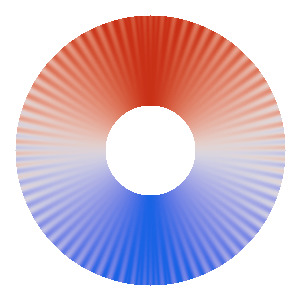
\includegraphics[width=4cm]{figures/CBWR_colourmap.jpg}
%\caption{}
\label{fig:CBWR_colourmap}
\end{figure*}

By default, a 1D colourmap is used. Aligned along the z-axis, spins in the \{0,0,1\} direction are red, while spins antiparallel to this \{0,0,-1\} are blue. Between these values, the colour transitions to white around the xy-plane. This corresponds to the "CBWR" colourmap, a cyclic blue-white-red map, which lends itself well to 1D or 2D spin sytems where there are two principle spin directions, such as antiferromagnets and ferrimagnets. Some care must be taken to align the principle spin directions with the z-axis, as this is the axis along which colour is applied. This can also be changed using the "-{}-vector-z" command line argument.   \\

\begin{figure*}[!h]
\center
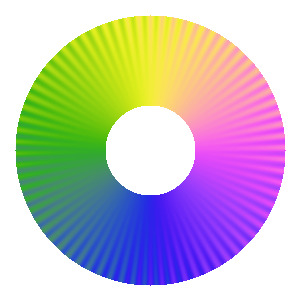
\includegraphics[width=4cm]{figures/C2_colourmap.jpg}
%\caption{}
\label{fig:C2_colourmap}
\end{figure*}

The "C2" coloumap is also cyclic and useful for 3D magnetic systems such as vortex states. It has four principle directions of magenta, yellow, green and blue. As it is cyclic, there will be a smooth transition between colour at all angles, irrespective of what is chosen as the zero degree spin direction. Sytems which benefit from this colourmap may also use the "-{}-3D" command line argument which applies a darkening and britening effect along the x-axis. \\

\begin{figure*}[!h]
\center

\includegraphics[width=7cm]{figures/BWR_colourmap.jpg}
%\caption{}
\label{fig:BWR_colourmap}
\end{figure*}

The "BWR" colourmap is very similar in properties to the CBWR map however it is not cyclic. This mean that spins along the positive z-axis will be red with a small positive y-component and blue with a small negative y-component. There will be an immediate flip from bright red to blue as this transition occurs. This can be used to emphasise the transition between spin directions. The transition point can be changed by using the "-{}-vector-z" command line argument. \\

\begin{figure*}[!h]
\center
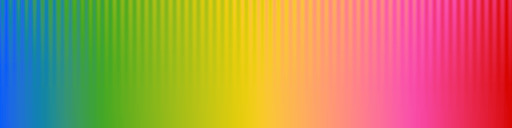
\includegraphics[width=7cm]{figures/Rainbow_colourmap.jpg}
%\caption{}
\label{fig:Rainbow_colourmap}
\end{figure*}

The "Rainbow" colourmap can be used in 2D systems where spins are aligned in many different directions such as high temperature simulations. While it is still designed to be somewhat perceptually uniform, this is very difficult to do with rainbow palettes hence its use typically loses detail when compared to other maps, however it is also one of the most vibrant. \\

\subsection*{Custom Colourmaps}

\begin{minipage}[c]{\textwidth}
\centering
\textit{vdc -{}-custom-colourmap [file-name]}
\end{minipage}\\

A user defined colourmap can also be used. To apply a different map, a file containing 256 colours in the RBG format must be provided in the same directory that vdc is run. RGB values must be space separated, with no other information such as line numbers. The beginning of an example colourmap is shown below. \\

Pregenerated perceptually uniform colourmaps of various forms, including those included in vampire by default, can be found in "peterkovesi.com/projects/colourmaps/index.html" under the Download secion. \\

\subsection*{custom\_colourmap\_file}
{\footnotesize
\begin{verbatim}
0.000000 0.000000 0.000000
0.005561 0.005563 0.005563
0.011212 0.011219 0.011217
0.016877 0.016885 0.016883
0.022438 0.022448 0.022445
0.027998 0.028011 0.028008
0.033540 0.033554 0.033551
0.039316 0.039333 0.039329
0.044700 0.044719 0.044714
0.049695 0.049713 0.049709
0.054322 0.054343 0.054338
\end{verbatim}
}

\subsection*{3D Systems}

\begin{minipage}[c]{\textwidth}
\centering
\textit{vdc -{}-3D}
\end{minipage}\\

POV-Ray images produced by vdc can have a 3D brightening effect applied by using the "-{}-3D" command line argument. When spins do not lie only in the yz-plane, their colour brightness is increased or reduced depending on their magnitude in the x-axis. \\

\subsection*{Defining axes}

\begin{minipage}[c]{\textwidth}
\centering
\textit{vdc -{}-vector-z x,y,z}
\end{minipage}\\

The principle axis along which colour is applied is the z-axis. This determines where colours will occur depending on the colour map being used. By default the "CBWR" map is used; spins along the positive z-direction are red, those along the negative z-direction are blue, and spins aligned along the xy-plane are white.\\

In many cases, the overall magnetic moment does not necessarily lie along the z-axis. To remedy this, a new "z-axis" may be defined. To redefine the z-axis, simply use the command "-{}-vector-z" followed by a direction vector. Note that this does not need to be normalised.\\

For example, if the user defines "-{}-vector-z 1,1,1", spins along the \{1,1,1\} direction will be red, \{-1,-1,-1\} will be blue and those perpendicular to the given axis will be white.\\

In some cases, the colourmap may not be symmetric along the default xy-plane, such as the "C2" colourmap. Here, spins along positive-y are magenta, while those antiparallel are green. This can be adjusted using a similar command line argument "-{}-vector-x", however this argument cannot be used without first defining "-{}-vector-z". \\

\section*{General customisation options}

There are several command line options that can be used to change all visualisation outputs including Rasmol, Jmol and POV-Ray. For example, it may be beneficial to use only smaller portions of your full system when generating POV-Ray or Rasmol images. This can help with large systems where rendering can become a time constraint, or systems made up of several elements which might be less relevant for the visualisation. There are several similar command line options which can be used to cut up the system in different ways:

\subsection*{Slice}

\begin{minipage}[c]{\textwidth}
\centering
\textit{vdc -{}-slice [xmin,xmax,ymin,ymax,zmin,zmax]}
\end{minipage}\\

The first slice type defines minimum and maximum values for each axis. Only atoms and spins inside these borders are included in the visualisation. The parameters passed to this argument are interpreted as fractional coordinates, hence a minimum of "0.0" and maximum "1.0" will include all atoms and spins. \\

By using this parameter, it is possible to halve a nanoparticle to see how spins at the centre of the system behave.\\

\subsection*{Void slice}

\begin{minipage}[c]{\textwidth}
\centering
\textit{vdc -{}-slice-void [xmin,xmax,ymin,ymax,zmin,zmax]}
\end{minipage}\\

Similar to "--slice", this parameter will \textit{remove} all atoms and spins inside the given borders. This can be used to create cubic hollow systems where only surface atoms are shown, possibly removing a very high percantage of atoms in the system, which can greatly reduce rendering time for both POV-Ray and Rasmol. \\

\subsection*{Sphere slice}

\begin{minipage}[c]{\textwidth}
\centering
\textit{vdc -{}-slice-sphere [xfrac,yfrac,zfrac]}
\end{minipage}\\

The sphere slice is also used to remove the atoms and spins at the centre of a system. This particular parameter lends itself well to spherical systems as it removes a spherical section of atoms. Three parameters are required, instead of six. Each one defines a region, centred on the centre of the original system, along the respective axis, equal to a fraction of the system size along that axis. As these parameters are not necessarily equal to each other, this can be used to create an ellipse of missing atoms at the centre of the system.

\subsection*{Cylindrical Slice}

\begin{minipage}[c]{\textwidth}
\centering
\textit{vdc -{}-slice-cylinder [xfrac,yfrac,zmin,zmax]}
\end{minipage}\\

Cylindrical systems are often surrounded by non-magnetic materials for parallelisation purposes. This slice parameter can be used to remove all atoms outside a cylindracal section by defining the x- and y-fractional sizes as well as a fractional minimum and maximum along the z-axis.

\subsection*{Remove materials}

\begin{minipage}[c]{\textwidth}
\centering
\textit{vdc -{}-remove-material [material1,material2,...]}
\end{minipage}\\

In some cases whole materials are not relevant for visualisation purposes and can be altogether removed. To use this command line parameter a list of material indices need to be provided. For example, to remove materials 2 and 4:

\begin{minipage}[c]{\textwidth}
\centering
\textit{vdc -{}-remove-material 2,4}
\end{minipage}\\

\subsection*{Antiferromagnetic materials}

\begin{minipage}[c]{\textwidth}
\centering
\textit{vdc -{}-afm [material1,material2,...]}
\end{minipage}\\

POV-Ray visualization of antiferromagnets can be difficult due to the contrast of colours of antiparallel spins. To remedy this, it is possible to define materials as antiferromagnetic. These materials will have their colours flipped so that they match neighbouring spins while their spin direction remains antiferromagnetic.

\section*{Micromagnetic visualization with PovRAY}
\addcontentsline{toc}{section}{Micromagnetic visualization with PovRAY}
cell2povray\\
macros\\
customization\\
colouring options\\

\section*{Visualization Movies}
\addcontentsline{toc}{section}{Visualization Movies}
